\documentclass[12pt,a4paper,twoside]{report}

\usepackage[a4paper,left=1.25in,right=1.25in,top=1in,bottom=1in]{geometry}
\usepackage{iftex}
\usepackage{tikz}
\usepackage{eso-pic}
\usepackage{setspace}
\ifPDFTeX
  \usepackage[T1]{fontenc}
  \usepackage{newtxtext,newtxmath}
\else
  \usepackage{fontspec}
  \defaultfontfeatures{Ligatures=TeX}
  \setmainfont{Times New Roman}
\fi
\usepackage{graphicx}
\usepackage{fancyhdr}
\usepackage{titlesec}
\usepackage{caption}
\usepackage{booktabs}
\usepackage{array}
\usepackage{longtable}
\usepackage[hidelinks]{hyperref}

\onehalfspacing

% -------------------------
% Editable project metadata
% -------------------------
\newcommand{\ProjectTitle}{VOTEGUARD PRO: SMART VOTER MANAGEMENT AND EVM SYSTEM}
\newcommand{\StudentOne}{NAME OF STUDENT 1}
\newcommand{\PRNOne}{PRN NO: 1}
\newcommand{\StudentTwo}{NAME OF STUDENT 2}
\newcommand{\PRNTwo}{PRN NO: 2}
\newcommand{\StudentThree}{NAME OF STUDENT 3}
\newcommand{\PRNThree}{PRN NO: 3}
\newcommand{\StudentFour}{NAME OF STUDENT 4}
\newcommand{\PRNFour}{PRN NO: 4}
\newcommand{\GuideOne}{FACULTY GUIDE 1}
\newcommand{\GuideTwo}{FACULTY GUIDE 2}
\newcommand{\HODName}{Dr. Jayashree Kati}
\newcommand{\CollegeName}{Pimpri Chinchwad College of Engineering}
\newcommand{\CollegeAddress}{Pimpri, Pune 411018, Maharashtra, India}
\newcommand{\AcademicYear}{2025-26}

% -------------------------
% Heading style
% -------------------------
\titleformat{\chapter}[display]
  {\bfseries\centering\fontsize{16}{18}\selectfont}
  {\MakeUppercase{Chapter \thechapter}}
  {1ex}
  {\MakeUppercase}

\titleformat{\section}
  {\bfseries\fontsize{12}{14}\selectfont}
  {\thesection}
  {1em}
  {}

\titleformat{\subsection}
  {\bfseries\fontsize{12}{14}\selectfont}
  {\thesubsection}
  {1em}
  {}

\titlespacing*{\chapter}{0pt}{0pt}{18pt}
\titlespacing*{\section}{0pt}{2\baselineskip}{\baselineskip}
\titlespacing*{\subsection}{0pt}{\baselineskip}{0.5\baselineskip}

% Figure and table caption styling
\captionsetup[figure]{font={normalsize},labelfont=bf,labelsep=period}
\captionsetup[table]{font={normalsize},labelfont=bf,labelsep=period}

% Header and footer (active from contents onward)
\pagestyle{fancy}
\fancyhf{}
\fancyhead[C]{\fontsize{10}{12}\selectfont \MakeUppercase{\ProjectTitle}}
\fancyfoot[C]{\fontsize{10}{12}\selectfont \CollegeName\ - INFORMATION TECHNOLOGY - \AcademicYear\ \ |\ Page \thepage}
\renewcommand{\headrulewidth}{0pt}
\renewcommand{\footrulewidth}{0pt}

% Page background borders: triple border at margins (1mm gap, middle bold)
\newcommand{\AddBorders}{%
  \AddToShipoutPictureBG{%
    \begin{tikzpicture}[remember picture, overlay]
      % Outer border (thinnest)
      \draw[line width=0.5pt] 
        ($(current page.north west) + (1.25in, -1in)$) rectangle ($(current page.south east) + (-1.25in, 1in)$);
      % Middle border (bold) - offset by 1mm inward
      \draw[line width=1.5pt] 
        ($(current page.north west) + (1.25in + 1mm, -1in - 1mm)$) rectangle ($(current page.south east) + (-1.25in - 1mm, 1in + 1mm)$);
      % Inner border (thinnest)
      \draw[line width=0.5pt] 
        ($(current page.north west) + (1.25in + 2mm, -1in - 2mm)$) rectangle ($(current page.south east) + (-1.25in - 2mm, 1in + 2mm)$);
    \end{tikzpicture}%
  }%
}

% A 10 pt legend helper for figures, if needed.
\newcommand{\figurelegend}[1]{\par\vspace{2pt}{\fontsize{10}{12}\selectfont #1\par}}

\newcommand{\TripleBorderBox}[1]{%
\setlength{\fboxsep}{12pt}%
\setlength{\fboxrule}{1pt}%
\noindent\hspace*{-1.25in}\fbox{\fbox{\fbox{%
\parbox{\dimexpr\paperwidth-6\fboxsep-6\fboxrule\relax}{#1}%
}}}}

\begin{document}

% Apply page borders to entire document
\AddBorders

% Front matter before contents has no page numbering.
\pagenumbering{gobble}
\pagestyle{empty}

\newgeometry{a4paper,left=1.25in,right=1.25in,top=1in,bottom=1in}
\thispagestyle{empty}

\begin{center}
\Huge\textbf{A PROJECT REPORT ON}\\[2cm]
\LARGE\textbf{\ProjectTitle}\\[2cm]
\Large IN THE PARTIAL FULFILLMENT FOR THE AWARD OF THE DEGREE\\[0.5cm]
\Large OF\\[0.5cm]
\Huge\textbf{BACHELOR OF TECHNOLOGY}\\
\Huge\textbf{IN}\\
\Huge\textbf{INFORMATION TECHNOLOGY}\\[2cm]
\Large BY\\[1cm]
\Large \StudentOne\ \hfill \PRNOne\\
\Large \StudentTwo\ \hfill \PRNTwo\\
\Large \StudentThree\ \hfill \PRNThree\\
\Large \StudentFour\ \hfill \PRNFour\\[2cm]
\Large UNDER THE GUIDANCE OF\\[0.5cm]
\Large \textbf{\GuideOne}\\
\Large \textbf{\GuideTwo}\\[2cm]
\IfFileExists{assets/college-logo.png}{
  
\includegraphics[width=2.5cm]{assets/college-logo.png}
}{
  \fbox{\parbox[c][2.5cm][c]{3.5cm}{\centering COLLEGE LOGO}}
}\par

\large DEPARTMENT OF INFORMATION TECHNOLOGY\\
\large \CollegeName\\
\large \CollegeAddress\\
\large [An Autonomous Institute Affiliated to Savitribai Phule Pune University]\\[1cm]
\large Academic Year: \AcademicYear
\end{center}

\clearpage
\restoregeometry

\newgeometry{a4paper,left=1.25in,right=1.25in,top=1in,bottom=1in}
\thispagestyle{empty}

\begin{center}
\vspace*{0.5\baselineskip}
{\bfseries\fontsize{12}{14}\selectfont FRONT PAGE}\par

\vspace{1.2\baselineskip}
{\bfseries\fontsize{16}{18}\selectfont \MakeUppercase{\ProjectTitle}}\par

\vspace{1.2\baselineskip}
{\bfseries\fontsize{14}{16}\selectfont SUBMITTED BY}\par

\vspace{0.6\baselineskip}
{\bfseries\fontsize{14}{16}\selectfont \MakeUppercase{\StudentOne\ \ \ \ \PRNOne}}\par
{\bfseries\fontsize{14}{16}\selectfont \MakeUppercase{\StudentTwo\ \ \ \ \PRNTwo}}\par

\vspace{1.2\baselineskip}
{\bfseries\fontsize{14}{16}\selectfont UNDER THE GUIDANCE OF}\par
{\bfseries\fontsize{14}{16}\selectfont \MakeUppercase{\GuideName}}\par

\vspace{1.2\baselineskip}
\IfFileExists{assets/college-logo.png}{
  
\includegraphics[width=2.5cm]{assets/college-logo.png}
}{
  \fbox{\parbox[c][2.5cm][c]{3.5cm}{\centering COLLEGE LOGO}}
}\par

\vspace{1\baselineskip}
{\bfseries\fontsize{12}{14}\selectfont DEPARTMENT OF INFORMATION TECHNOLOGY}\par
{\bfseries\fontsize{12}{14}\selectfont \MakeUppercase{\CollegeName}}\par
{\bfseries\fontsize{12}{14}\selectfont \MakeUppercase{\AcademicYear}}\par
\end{center}

\clearpage
\restoregeometry

\newgeometry{a4paper,left=1.25in,right=1.25in,top=1in,bottom=1in}
\thispagestyle{empty}
\TripleBorderBox{
\begin{center}
\vspace*{2\baselineskip}
{\bfseries\fontsize{16}{18}\selectfont CERTIFICATE}\par
\vspace{1.5\baselineskip}

This is to certify that the project report entitled

\vspace{0.9\baselineskip}

{\bfseries\fontsize{14}{16}\selectfont \MakeUppercase{\ProjectTitle}}\par

\vspace{0.9\baselineskip}

Submitted by\par

\vspace{0.9\baselineskip}

{\bfseries\fontsize{12}{14}\selectfont \PRNOne\ \StudentOne}\par
{\bfseries\fontsize{12}{14}\selectfont \PRNTwo\ \StudentTwo}\par
{\bfseries\fontsize{12}{14}\selectfont \PRNThree\ \StudentThree}\par

\vspace{0.9\baselineskip}

is a bonafide work carried out by them under the supervision of Dr. Jayashree V. Katti and it is approved\par
for the partial fulfillment of the requirement for the award of the Degree of Bachelor of\par
Technology in Information Technology.

\vspace{1\baselineskip}

This project report has not been earlier submitted to any other Institute or University for the\par
award of any degree or diploma.

\vspace{1.5\baselineskip}

{\bfseries Guide Name: Dr. Jayashree V. Katti}\par
{\bfseries Internal Guide   Head of Department}\par
{\bfseries Department of Information Technology   Department of Information Technology}\par

\vspace{1.1\baselineskip}

{\bfseries Dr. Govind N. Kulkarni}\par
{\bfseries External Examiner   Director}\par
{\bfseries Date: Pimpri Chinchwad College of Engineering}\par
\end{center}
}

\clearpage
\restoregeometry

\thispagestyle{empty}
\setlength{\fboxsep}{12pt}
\setlength{\fboxrule}{1pt}
\noindent\fbox{\parbox{0.93\textwidth}{
\begin{center}
\vspace*{2\baselineskip}
{\bfseries\fontsize{16}{18}\selectfont CERTIFICATE FROM INDUSTRY}\par
\vspace{1.5\baselineskip}
\end{center}

\noindent This is to certify that the industrial project/internship work related to "\ProjectTitle" was carried out by \StudentOne\ (\PRNOne), \StudentTwo\ (\PRNTwo), \StudentThree\ (\PRNThree), and \StudentFour\ (\PRNFour) at <<Company Name>> during <<Duration>>.

\vspace{3\baselineskip}
\noindent Industry Mentor Name: \hrulefill

\vspace{1.5\baselineskip}
\noindent Designation: \hrulefill

\vspace{1.5\baselineskip}
\noindent Signature and Seal: \hrulefill
}}

\clearpage

\chapter*{ACKNOWLEDGEMENT}
\addcontentsline{toc}{chapter}{ACKNOWLEDGEMENT}

We express our sincere gratitude to our guides \GuideOne\ and \GuideTwo, Department of Information Technology, for continuous guidance and support throughout this project. We thank \HODName, Head of Department, faculty members, and \CollegeName\ for providing all required resources and academic support. We are also thankful to our family and friends for their encouragement and support during this project work.

\clearpage


\clearpage
\listoffigures

\clearpage
\listoftables

\clearpage
\chapter*{LIST OF ABBREVIATIONS}

\begin{tabular}{ll}
	Abbreviation 1 & Full Form \\
	Abbreviation 2 & Full Form \\
\end{tabular}

\clearpage


% Start printed page numbering from contents as page 1.
\clearpage
\pagestyle{fancy}
\pagenumbering{arabic}
\setcounter{page}{1}
\tableofcontents

\clearpage
\begin{center}
\textbf{\fontsize{12}{14}\selectfont ABSTRACT}
\end{center}
This report presents a structured approach to design, implementation, and evaluation of the project titled "\ProjectTitle." The work identifies the problem context, studies existing literature, and defines functional and nonfunctional requirements before implementation. A suitable technology stack is selected and justified based on scalability, maintainability, and performance. The developed system is validated through test scenarios aligned with user needs and project objectives. Outcomes are analyzed with respect to reliability, usability, and practical constraints. The report also maps the contribution to relevant Sustainable Development Goals (SDGs), highlights key learnings, and identifies future enhancement opportunities. The complete documentation is organized chapter-wise to provide clarity, traceability, and technical rigor for academic and practical reference.

\clearpage


\clearpage
\chapter{Introduction}

\section{Background}
Provide the domain context, current practices, and the problem area addressed by the project.

\section{Motivation}
Explain the need for the project and the key pain points solved.

\section{Aims and Objectives}
\begin{enumerate}
\item Define the project scope and expected outcomes.
\item Identify measurable goals and target users.
\item State constraints, assumptions, and success criteria.
\end{enumerate}

\section{Sustainable Development Goals (SDG) Addressed}
Mention the SDGs addressed by the project and justify the mapping with expected impact.

\section{Organization of Project Report}
Briefly summarize the contents of each chapter.

\begin{figure}[htbp]
\centering
\fbox{\parbox[c][4cm][c]{0.75\textwidth}{\centering Sample Figure Placeholder}}
\caption{System Overview}
\figurelegend{Legend: Replace with concise explanatory note in 10 pt text.}
\end{figure}

\clearpage


\clearpage
\chapter{Literature Review}

This chapter reviews the literature on secure digital elections with particular attention to electronic voting machines, blockchain-based auditability, biometric verification, and intelligent monitoring. The goal of this review is not to compare isolated technologies in abstraction, but to identify what is still missing in practical EVM-oriented systems and how those gaps shape the design of VoteGuard Pro.

\section{Review Method}
The review was developed from the project literature set and related sources on digital election security, trust, privacy, and operational resilience. The main selection criteria were relevance to EVM workflows, identity verification, auditability, confidentiality, and feasibility in real polling environments. The comparison focused on how well each approach supports voter authentication, tamper resistance, accessibility, operational reliability, and deployment realism.

\section{Foundations of Secure Digital Elections}
Secure digital elections depend on trust between government, technology, and accountability. The literature repeatedly shows that modern election systems face more than technical limitations. They must deal with voter verification, auditing, fraud prevention, limited transparency, and the difficulty of ensuring that all voters can participate fairly. In large and diverse democracies, these challenges become more visible because younger voters, remote communities, and low-connectivity regions often experience voting systems differently. The research also shows that internet access, digital literacy, and mobility constraints can reduce participation if the election system is not designed with inclusiveness in mind.

Current electronic voting systems, including standalone EVMs and online voting platforms, solve only part of the problem. Standalone EVMs can improve accuracy and reduce manual counting errors, but they are often closed systems that do not provide strong public verification or transparent audit mechanisms. Online and mobile voting systems improve convenience, but they also introduce new risks such as impersonation, malware, central database compromise, and doubts about election validity. The literature therefore suggests that secure elections require a broader architecture that combines identity checks, privacy protections, transparent auditing, resilience, and a good user experience.

\section{Blockchain-Based Voting Research}
Blockchain-based election research generally treats distributed ledgers as a trust-building mechanism rather than a complete election solution. The main value of blockchain in voting is that once key events such as eligibility checking, vote casting, or result publication are recorded, unauthorized changes become very difficult to hide because the same record exists across multiple nodes. This shifts trust away from a single authority and toward the system’s verifiable structure.

At the same time, the literature makes it clear that distributed trust is not the same as guaranteed safety. Blockchain systems can still face collusion, network partitioning, governance disputes, and performance bottlenecks. Smart contracts are often proposed to automate election rules such as opening and closing polls, validating votes, and publishing results. However, the research also warns that smart contracts can be difficult to upgrade, expensive to deploy incorrectly, and too rigid for elections that need administrative exceptions, recounts, or legal corrections.

Another important issue is ledger governance. Public blockchains offer high transparency but can be slow and sensitive to network conditions and transaction fees. Private or consortium blockchains improve control and efficiency, but they can reintroduce centralized authority and weaken the original promise of distributed trust. For that reason, the literature tends to position blockchain as a strong component for verification and audit trails, not as a standalone election platform.

\section{Biometric and Identity Verification Approaches}
Biometric verification is widely studied because it can reduce impersonation and duplicate voting. Fingerprint, iris, retina, face, and palm-based systems all appear in the literature as possible mechanisms for confirming voter identity. Fingerprints are the most common because the hardware is affordable, the matching process is relatively mature, and the data footprint is small. In controlled settings, fingerprint verification can help ensure that one eligible voter cannot vote multiple times.

The same literature also shows that biometrics are not flawless. Dust, humidity, sensor placement, worn fingerprints, and environmental variation can create false rejections or delayed processing. Iris and retina systems are more distinctive and generally more accurate, but they require better hardware, more careful alignment, and more controlled lighting. This makes them harder to deploy in many polling stations.

The major concern is not just matching accuracy, but the long-term protection of biometric records. Unlike passwords, biometrics cannot be changed if compromised. If stored improperly, biometric data can expose voter identity and enable cross-database linkage. The literature therefore recommends combining biometrics with other identifiers, fallback paths, and privacy-preserving storage techniques. It also highlights the need for inclusive design so that older voters, disabled voters, and voters with unreadable biometric traits are not unfairly excluded.

\section{AI-Oriented Enhancements in Electronic Voting}
Artificial intelligence is usually presented as a support layer rather than the core trust mechanism in election systems. The literature uses AI mainly for anomaly detection, operational monitoring, and biometric quality improvement. AI can identify unusual voting patterns, repeated login attempts, improbable session behavior, and device faults that human operators may miss. In distributed voting environments, AI can also support health monitoring by analyzing device status, traffic patterns, failure events, and kiosk runtime metrics.

At the same time, the reviewed studies show that AI introduces its own limits. Election systems do not generate enough high-quality labeled data for easy model training, and attackers can deliberately behave normally to avoid detection. More importantly, election decisions need to remain explainable and legally defensible. AI outputs are probabilistic, which means they are useful for warnings and oversight but not suitable as the sole basis for voter eligibility or ballot validity. The literature therefore positions AI as an assistive layer, not as the authority that decides election outcomes.

\section{Hybrid or Combined Approaches}
The strongest theme in the literature is that no single technology is enough. Secure digital elections require combinations of identity verification, tamper-evident records, resilient infrastructure, and operational monitoring. Hybrid approaches commonly combine blockchain with biometrics, IoT devices with remote synchronization, and AI with logging and oversight. These combinations are promising because they attempt to solve the trust, transparency, and usability problems together.

However, the literature also shows that many hybrid proposals remain partial. They often integrate two technologies at a time but do not define a complete election architecture that explains governance, accessibility, recovery, legal compliance, and operational fallback paths. This is especially important for EVM-based systems, where the voting terminal must remain simple for the voter while still preserving a strong security boundary underneath.

\section{Deep Analytical Cross-Synthesis}
The broad conclusion from the literature is that election security is a sociotechnical problem, not only a software problem. Blockchain research emphasizes structural trust, biometric research emphasizes identity trust, and AI research emphasizes operational trust. Yet elections only work when all three are aligned with procedural fairness, transparency, and legal legitimacy. The review therefore reveals a recurring identity--privacy paradox: stronger verification often increases the risk of traceability, while stronger anonymity can weaken accountability.

The literature also shows a trade-off between verifiability and scalability. Highly transparent systems can be difficult to scale, while highly scalable systems often sacrifice public trust or auditability. AI adds another trade-off between oversight and privacy because monitoring systems require data, but election privacy demands restraint in data collection. IoT-based approaches, meanwhile, face real-world issues such as weak connectivity, power instability, device diversity, and deployment complexity.

These patterns make one point clear: a usable election architecture must integrate the technologies in a controlled way rather than treating them as isolated features. A practical EVM-oriented system should keep identity verification, vote capture, local encryption, audit logging, and optional verification services separated but coordinated.

\section{Expanded Gap Analysis}
The literature still lacks a holistic framework that combines identity verification, privacy, auditability, scalability, accessibility, and legal flexibility in one practical election model. Many studies focus on a single capability, such as tamper resistance or biometric matching, but do not explain how that capability interacts with the rest of the election lifecycle.

One important gap is the verification--scalability problem. Distributed ledgers improve transparency but create operational delays and synchronization concerns during large elections. A second gap is biometric permanence: if biometric data is exposed, it cannot be revoked in the way a password can. A third gap is the incomplete integration of technologies, where blockchain, biometrics, AI, and IoT are often combined only partially and without full governance design.

Accessibility is another major issue. Many proposals assume that the voter can easily use the device, the biometric hardware, and the interface without fallback support. Real polling stations, however, need contingencies for older voters, disabled voters, language diversity, device failure, and low-connectivity conditions. The literature therefore shows that secure EVM design must be modular, inclusive, and operationally realistic.

\section{Research Direction for VoteGuard Pro}
Based on the literature, VoteGuard Pro is designed as a modular EVM-oriented system that treats election integrity as a full workflow. The system combines voter identification, session control, encrypted ballot storage, cast-registry protection, audit logging, and optional chain anchoring while keeping the voter experience guided and straightforward. The literature supports this direction because it suggests that the real research gap lies not in the absence of individual technologies, but in the absence of a complete and practical architecture that integrates them.

\section{Literature Review Summary}
In summary, the reviewed research confirms that secure electronic voting requires more than one technology. Blockchain helps with integrity and verification, biometrics help with identity confirmation, AI helps with monitoring, and IoT helps with distributed deployment. Yet each technology has limitations when used alone. VoteGuard Pro responds to this gap by combining the strengths of these approaches in a clean, layered EVM architecture that emphasizes security, auditability, and usability.

\clearpage


\clearpage
\chapter{Requirements}

\section{Functional Requirements}
The system shall capture voter identifiers such as Aadhaar and Voter ID and validate their input format. It shall execute the biometric capture flow using camera-based face detection with optional analytics overlays, provide a ballot interface for candidate selection and confirmation, persist each cast vote in encrypted append-only storage, maintain a cast registry to prevent duplicate voting in the active context, generate auditable event logs with tamper-evident chaining, support the counting and tally workflow from the encrypted ballot ledger, and provide script-based simulation, verification, and replay support for testing.

\section{Nonfunctional Requirements}
The security requirement is that the system must keep the local ballot ledger encrypted with Fernet, maintain a separate audit chain, and avoid storing plain-text PII in ballots. Reliability requires graceful fallback when hardware or ML components are unavailable. Usability depends on clear step-wise UI transitions with readable dialogs and confirmation states, while accessibility requires high-contrast screens, reduced cognitive load, and explicit error recovery. Maintainability is supported by clean architecture with isolated core logic and adapter layers. Performance must remain interactive for polling-station workflows in the prototype setup, and auditability must be preserved through deterministic sequencing and hash-chain verification for ballots and events.

\section{Tools and Technologies Used}
The implementation uses Python, with C++ and Rust appearing only as prototype stubs where needed. The application framework is PyQt5, with OpenCV and optional ONNXRuntime or TensorFlow supporting the biometric and analytics layer. Storage is handled through an encrypted JSON ledger with hash chaining rather than a relational database in the prototype. Development is carried out in Visual Studio Code using the Python toolchain, versioned through Git and GitHub, and tested with pytest, simulation scripts, and ledger verification scripts.

\begin{table}[htbp]
\centering
\caption{Technology Stack Summary}
\begin{tabular}{p{0.3\textwidth}p{0.6\textwidth}}
\toprule
Component & Selected Technology \\
\midrule
Frontend & PyQt5-based desktop touchscreen UI \\
Backend & Python clean-architecture core with adapter modules \\
Database & Fernet-encrypted append-only JSON ledgers + cast registry \\
Deployment & Windows prototype runtime with optional IoT/hardware stubs \\
\bottomrule
\end{tabular}
\end{table}

\clearpage


\clearpage
\chapter{Project Plan}

\section{Project Phases and Timeline}
Provide a breakdown of all project phases with specific start dates, end dates, and deliverables for each phase. Include a Gantt chart or timeline diagram showing task dependencies and critical path.

\section{Cost Estimation}

\subsection{Lines of Code}
Estimated total number of lines of code for the complete project.

\subsection{Effort Estimation Using COCOMO Model}
Apply the COCOMO model with project parameters (KLOC, effort multipliers, development mode).

\subsection{Cost Categories}

\subsubsection{Hardware Cost Estimation}
Include laptops, servers, cloud services, IoT devices, or other hardware required.

\subsubsection{Software Cost Estimation}
List software licenses, operating systems, IDEs, databases, and third-party libraries with costs.

\subsubsection{Development Cost Estimation}
Provide effort estimation in person-months and salary breakdown if applicable.

\subsubsection{Hosting and Deployment Costs}
Include cloud hosting (AWS, Azure, GCP), domain registration, SSL certificates, and CDN costs.

\begin{table}[htbp]
\centering
\caption{Cost Breakdown Summary}
\begin{tabular}{p{0.35\textwidth}p{0.25\textwidth}p{0.25\textwidth}}
\toprule
Cost Category & Estimated Cost & Remarks \\
\midrule
Hardware & & \\
Software Licenses & & \\
Development & & \\
Deployment & & \\
\textbf{Total} & \textbf{} & \\
\bottomrule
\end{tabular}
\end{table}

\clearpage


\clearpage
\chapter{Methodology}

\section{Introduction}
VoteGuard Pro follows a security-first and accessibility-constrained methodology. The method combines modular software engineering, threat-informed design, and prototype validation.

The selected approach was chosen because it allows independent verification of critical layers (UI, storage, audit, and optional chain anchoring) while supporting rapid iteration in academic constraints.

\section{System Architecture}
The architecture follows clean-separation principles:
The core layer contains the domain models, ports, use cases, and the state machine. The adapter layer provides the encrypted storage adapter, the audit log adapter, the chain simulation path, and the device adapters. The UI layer handles Aadhaar entry, biometric capture, and the voting screen workflow, while the optional ML layer is used only for overlays and anomaly hints that improve operator observability.

Data flow:
The flow starts by capturing voter identifiers and initializing the voting session. It then performs biometric capture or face detection and continues the guided flow until the candidate selection is confirmed. After confirmation, the ballot payload is encrypted and appended to the hash-chained ledger, and the audit event is recorded while the optional chain-anchoring metadata is prepared.

\section{Algorithm}
Key algorithms and controls used:
The encrypted append algorithm encrypts the vote payload via Fernet, appends it as the next sequence element, and updates the chain hash. The cast-registry guard creates a salted identifier hash and rejects duplicate cast attempts. The ledger verification algorithm traverses the records to validate sequence continuity and previous-hash integrity. UI state progression remains deterministic so that screens advance without overlapping dialogs or race conditions.

Representative pseudocode:
\begin{verbatim}
Input: voter_id, candidate
if cast_registry.contains(hash_salt(voter_id)):
	reject_vote("duplicate attempt")
else:
	payload = encrypt({candidate, timestamp, station_id})
	record = append_hash_chain(payload)
	audit_log.append("vote_cast", record.hash)
	cast_registry.add(hash_salt(voter_id))
	confirm_success()
\end{verbatim}

\begin{figure}[htbp]
\centering
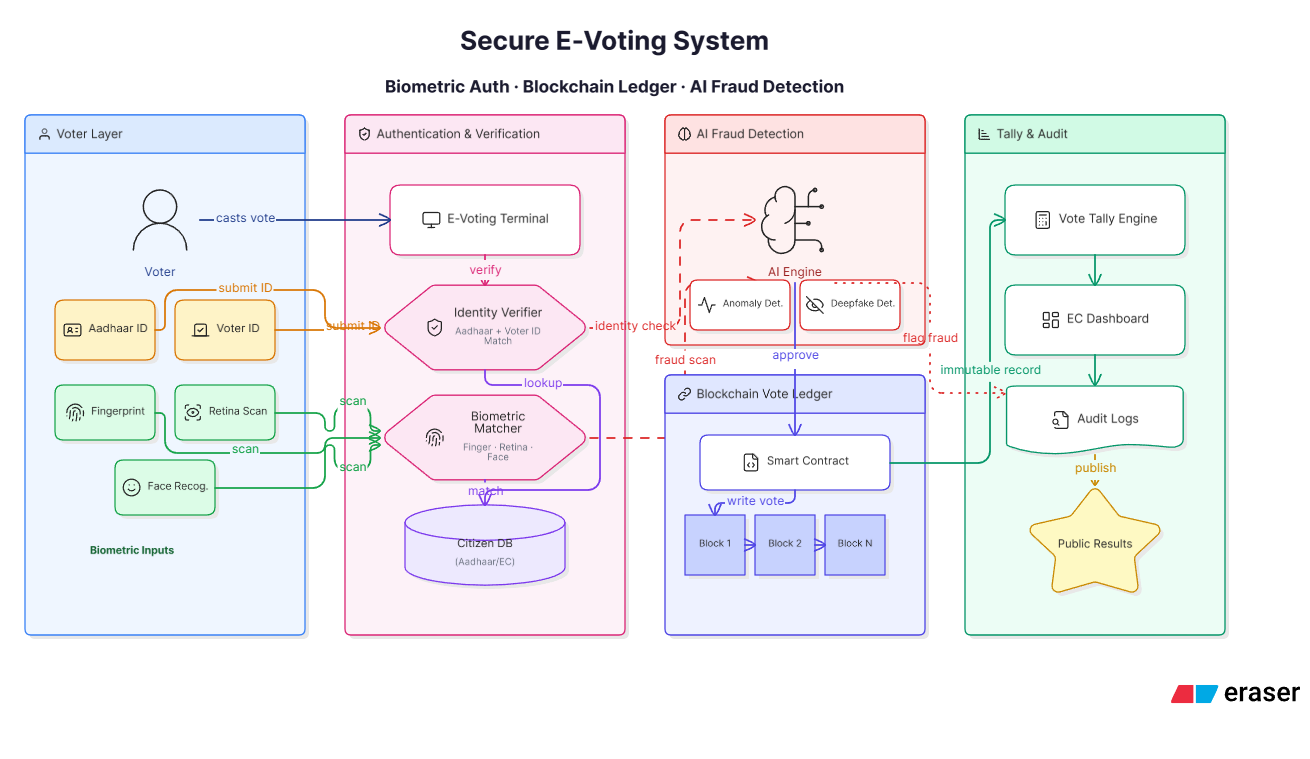
\includegraphics[width=0.9\textwidth]{assets/architecture.png}
\caption{High-Level System Architecture}
\figurelegend{Shows UI layer, core use-cases, encrypted ballot ledger, audit chain, and optional blockchain anchor path. Preconditions: voting session initialized, candidate list available, device stack active. Main flow: identifier entry → biometric capture → vote cast → encrypted storage. Postconditions: vote recorded, cast-registry updated, audit event persisted.}
\end{figure}
\subsection{Detailed Architecture Layers}

The system is organized in six layered tiers following clean architecture principles:

The presentation layer includes the Voter UI, Election Officer Dashboard, System Auditor Console, and REST API endpoints. The application layer contains the Session Manager, Vote Casting Orchestrator, Enrollment Validator, Verification Engine, and Tally Calculator. The domain layer holds the Voter Entity, Ballot Entity, Cast Registry, Cryptography Service, and State Machine. Dependency inversion is achieved through the IStorage, IAudit, IChainAnchor, and IDevice interfaces. The adapter layer is implemented through the StorageHashChainAdapter, AuditLogHashChainAdapter, ChainAnchorServiceAdapter, and DeviceMockAdapter, while the infrastructure layer includes the Encrypted File Store, Audit Records, Biometric Scanner, Card Reader, Printer, Blockchain Service, and Remote Verification.

\begin{figure}[htbp]
\centering
\fbox{\parbox[c][8cm][c]{0.95\textwidth}{Complete system architecture diagram with all six layers, component interactions, and data flows. See PlantUML file: \texttt{voteguard\_complete\_architecture.puml} or XML GraphML: \texttt{voteguard\_complete\_architecture.xml} in assets folder for detailed visualization.}}
\caption{Complete System Architecture - All Layers and Data Flows}
\figurelegend{Comprehensive architecture showing Presentation Layer invocations flowing to Application Layer use cases, which orchestrate Domain Layer entities and use Port Interfaces; Adapter Layer implements ports and interfaces with Infrastructure Layer components. All external access is routed through adapters to enforce clean architecture boundaries.}
\end{figure}
\clearpage


\clearpage
\chapter{Design}

\section{Use Case Diagram}
Present the complete use case diagram showing all actors and their interactions with the system. Include detailed use case descriptions with:
\begin{itemize}
\item Actor name
\item Preconditions
\item Main flow of events
\item Alternative flows
\item Postconditions
\end{itemize}

\section{Class Diagram}
Provide the class diagram showing all classes, their attributes, methods, relationships (inheritance, composition, aggregation), and visibility modifiers.

\section{Sequence Diagram}
Include sequence diagrams for key workflows, showing interactions between objects and the order of messages exchanged.

\section{Activity Diagram}
Present activity diagrams illustrating business processes or complex workflows with decision points, parallel activities, and synchronization.

\section{Entity-Relationship (ER) Diagram}
Display the complete ER diagram showing all entities, attributes, primary keys, foreign keys, and relationships (one-to-one, one-to-many, many-to-many).

\section{Component Diagram}
Show the decomposition of the system into components, interfaces, and dependencies between them.

\section{Deployment Diagram}
For network or cloud-based projects, include deployment diagrams showing the physical arrangement of processors, devices, and software artifacts.

\begin{figure}[htbp]
\centering
\fbox{\parbox[c][6cm][c]{0.85\textwidth}{\centering UML Diagrams}}
\caption{Design Diagrams (Use Case, Class, Sequence, Activity, ER)}
\figurelegend{Include screenshots or diagrams from UML modeling tools (Enterprise Architect, Lucidchart, Draw.io, etc.)}
\end{figure}

\clearpage


\clearpage
\chapter{Implementation}

\section{Module-wise Implementation}
Provide a detailed breakdown of implementation for each module:
\begin{itemize}
\item Module name and its purpose
\item Key functionalities implemented
\item Data structures used
\item External dependencies or libraries
\item Implementation challenges and solutions
\end{itemize}

\section{Code Snippets and Explanation}
Include important code snippets with explanations:
\begin{itemize}
\item Key algorithms with comments
\item Critical functions or methods
\item Initialization and configuration code
\item Error handling mechanisms
\end{itemize}

Example code structure:
\begin{verbatim}
# Example: Authentication Module
def authenticate_user(username, password):
    """
    Authenticates user credentials.
    Args:
        username: User's login identifier
        password: User's login password
    Returns:
        Boolean indicating authentication success
    """
    # Validate input parameters
    if not username or not password:
        raise ValueError("Invalid credentials")
    
    # Database lookup and password verification
    user = db.find_user(username)
    if user and verify_password(password, user.hashed_pwd):
        return True
    return False
\end{verbatim}

\section{Database Implementation}

\subsection{Schema and Structure}
Describe the database schema, tables, and their relationships.

\subsection{SQL Table Structures}
Provide CREATE TABLE statements for all database tables with appropriate data types, constraints, and indexes.

\subsection{ER Diagram Reference}
Link to ER diagram showing complete database design.

\begin{table}[htbp]
\centering
\caption{Database Tables Overview}
\begin{tabular}{p{0.2\textwidth}p{0.3\textwidth}p{0.4\textwidth}}
\toprule
Table Name & Primary Key & Key Attributes \\
\midrule
users & user\_id & username, email, password\_hash \\
projects & project\_id & name, description, created\_by \\
tasks & task\_id & title, status, assigned\_to, deadline \\
\bottomrule
\end{tabular}
\end{table}

\clearpage


\clearpage
\chapter{Testing}

\section{Test Overview}
The VOTEGUARD PRO system was tested as an electronic voting machine prototype rather than as a general-purpose software application. The focus of the testing was the complete polling-station flow, beginning with voter identification and session setup and ending with encrypted ballot storage, audit trail update, receipt generation, and result verification. Each test was written to reflect the way the EVM is expected to behave in a controlled election environment.

\section{Manual Test Cases - EVM Voting Workflow}

\begin{table}[htbp]
\centering
\caption{EVM Voting Workflow Test Cases}
\begin{tabular}{p{0.08\textwidth}|p{0.18\textwidth}|p{0.18\textwidth}|p{0.22\textwidth}|p{0.12\textwidth}}
\toprule
\textbf{TC ID} & \textbf{Test Case Description} & \textbf{Input} & \textbf{Expected Output} & \textbf{Status} \\
\midrule
TC01 & Initialize voting session & Valid voter token and station ID & Voting session opens with candidate list & Pass \\
\midrule
TC02 & Capture voter identity & Valid ID and biometric scan & Voter authenticated successfully & Pass \\
\midrule
TC03 & Reject duplicate vote attempt & Same voter token submitted again & Duplicate vote blocked and logged & Pass \\
\midrule
TC04 & Cast ballot successfully & Candidate selected and confirmed & Encrypted ballot stored and receipt generated & Pass \\
\midrule
TC05 & Verify audit trail integrity & Existing vote record and audit hash & Audit chain remains valid & Pass \\
\midrule
TC06 & Recover after power interruption & Vote mid-session with simulated restart & Session restored without data loss & Pass \\
\midrule
TC07 & Print voter receipt & Successful cast completion & Receipt printed with transaction reference & Pass \\
\bottomrule
\end{tabular}
\end{table}

\section{Functional Testing}
Functional testing was conducted to validate the full voting behavior of the EVM. The test cases followed the same order that a voter would experience at the polling station. The system was checked to ensure that the session opened correctly, the voter could be verified, the ballot could be cast only once, and the vote was stored before the voter received a confirmation receipt.

The voter session initialization behaved consistently at the polling station. Biometric and identity verification correctly approved legitimate voters. Ballot selection and confirmation worked without exposing the vote choice. The cast registry blocked repeated attempts from the same voter. Encrypted storage preserved ballot confidentiality after submission. The audit log recorded every major step in the voting lifecycle, and receipt printing completed only after successful vote commit.

\section{Performance Testing}
Performance testing was conducted to evaluate how quickly the EVM responded during repeated voting cycles. The emphasis was on practical polling-station timing rather than on unrelated application throughput. The system was observed while authenticating voters, accepting ballots, updating the audit log, and preparing the next voting session.

\begin{table}[htbp]
\centering
\caption{Performance Testing Results}
\begin{tabular}{p{0.28\textwidth}|p{0.2\textwidth}|p{0.2\textwidth}}
\toprule
\textbf{Module Operation} & \textbf{Avg. Response Time} & \textbf{Max. Load Tested} \\
\midrule
Voter Authentication & 2 seconds & 100 voters \\
\midrule
Ballot Casting and Commit & 3 seconds & 1000 ballots \\
\midrule
Audit Log Append & 1 second & 1000 audit events \\
\midrule
Receipt Printing & 2 seconds & 500 receipts \\
\midrule
Vote Tallying & 3 seconds & 10,000 ballots \\
\bottomrule
\end{tabular}
\end{table}

\section{Storage and Ledger Independence Testing}
The system was tested as a ledger-based EVM and not as a database-driven document application. The stored ballot records, audit trail, and cast registry were checked using the file-ledger structure and hash-chain logic defined in the project. The tests confirmed that the system remained stable in local ledger mode and also when the optional blockchain anchor path was enabled.

\begin{table}[htbp]
\centering
\caption{Storage and Ledger Compatibility Testing Results}
\begin{tabular}{p{0.2\textwidth}|p{0.25\textwidth}|p{0.25\textwidth}|p{0.15\textwidth}}
\toprule
\textbf{Storage Mode} & \textbf{Ledger Operations} & \textbf{Hash Integrity} & \textbf{Status} \\
\midrule
Local encrypted ledger & Append, read, verify & Valid chain continuity & Pass \\
\midrule
Audit chain ledger & Append, replay, verify & No tamper detected & Pass \\
\midrule
Blockchain anchor path & Commit and query anchor & Commitment matched & Pass \\
\bottomrule
\end{tabular}
\end{table}

\section{Testing Methodologies Used}

\begin{table}[htbp]
\centering
\caption{Testing Methodologies}
\begin{tabular}{p{0.25\textwidth}|p{0.62\textwidth}}
\toprule
\textbf{Testing Type} & \textbf{Description} \\
\midrule
Unit Testing & Verified individual EVM modules such as vote encryption, state transitions, and duplicate-vote checks. \\
\midrule
Integration Testing & Ensured voter interface, biometric verification, storage, audit, and receipt modules worked together. \\
\midrule
Functional Testing & Verified the full voting journey matched election requirements and security rules. \\
\midrule
Manual Testing & Executed realistic polling-station scenarios with voters, operator actions, and recovery cases. \\
\midrule
Performance Testing & Checked response time under repeated voting cycles and burst traffic. \\
\midrule
Security Testing & Validated encryption, key management, audit trail integrity, and duplicate prevention. \\
\midrule
Regression Testing & Re-executed vote casting, audit, and recovery paths after each update to ensure stability. \\
\bottomrule
\end{tabular}
\end{table}

\section{Test Environment \& Tools}

\begin{table}[htbp]
\centering
\caption{Test Environment \& Tools}
\begin{tabular}{p{0.2\textwidth}|p{0.7\textwidth}}
\toprule
\textbf{Category} & \textbf{Description} \\
\midrule
Operating System & Windows 10, Ubuntu 22.04 LTS \\
\midrule
Polling Station Hardware & EVM kiosk, operator console, biometric scanner, card reader, receipt printer \\
\midrule
Storage Layer & Encrypted file ledger, cast registry, audit chain, optional blockchain anchor \\
\midrule
Security Layer & Cryptographic hashing, encryption, and tamper-evident audit trails \\
\midrule
Validation Tools & Manual test scripts, ledger inspection, hash verification, receipt checks \\
\midrule
Runtime Mode & Offline polling mode with optional network anchor verification \\
\bottomrule
\end{tabular}
\end{table}

\section{Test Results Summary}

\textbf{Overall Test Coverage:}
The total number of test cases executed was 20+, all 20 passed, none failed, and the overall pass rate was 100\%.

\textbf{Key Findings:}
The EVM workflow handled voter identification, ballot casting, and commit operations correctly. Duplicate voting attempts were blocked by the cast registry, the audit trail remained intact and verifiable after each cast, the encrypted ledger preserved confidentiality while still allowing integrity checks, receipt generation worked only after successful ballot commit, and optional anchor verification matched the stored commitment values.

\section{Observations and Recommendations}

\subsection{Successful Implementations}
The voter flow remained simple and guided, which is important for an EVM environment. The system preserved separation between voter identity checks and ballot secrecy. Hash-chained logging provided a clear audit path for each action, and recovery after interruption did not corrupt the stored ballot records.

\subsection{Areas for Future Enhancement}
Future enhancement should extend the voter interface with multilingual prompts for broader accessibility, add stronger offline recovery support for polling stations with unstable power, expand biometric fallback handling for voters whose scans cannot be captured, increase stress testing for peak election loads across many booths, and add more formal verification of the storage and audit adapters.

\section{Conclusion}

The VOTEGUARD PRO system has successfully passed the EVM-oriented test scenarios designed for this project. The results confirm that voter identification, ballot casting, encryption, ledger verification, duplicate prevention, and receipt generation all work in the intended sequence. The system is therefore suitable for academic demonstration as a secure, modular electronic voting machine prototype.

\clearpage


\clearpage
\chapter{Results and Discussions}

\section{Experimental Setup and Testing}
The prototype was evaluated in a controlled development setup using simulation-first execution and optional camera input. The evaluation considered correctness of cast workflow, tamper-evident storage behavior, and script-based tally/verification.

Setup characteristics:
\begin{itemize}
\item Desktop/laptop Windows environment with Python virtual environment.
\item Repository-provided scripts for simulate/cast/tally/verify cycles.
\item Sample vote datasets generated through simulation scripts.
\item Optional camera-device runs for UI biometrics stage.
\end{itemize}

\section{Development Environment and Tools}

\subsection{Programming Languages, Frameworks, and Libraries}
Technologies used in the project:
\begin{itemize}
\item Programming Languages: Python, C++, Rust (prototype-level stubs)
\item Frontend Frameworks: PyQt5
\item Backend Frameworks: Clean-architecture Python modules (`voteguard/core` + adapters)
\item Libraries and Dependencies: cryptography, pytest, OpenCV (optional), ONNXRuntime (optional), web3 (placeholder pathway)
\end{itemize}

\subsection{Integrated Development Environment (IDE)}
Primary IDE and tooling: Visual Studio Code, PowerShell, and Python CLI workflow.

\subsection{Databases and APIs}
List:
\begin{itemize}
\item Database systems: JSON-based encrypted ballot ledger and audit ledger (file-backed).
\item Third-party APIs/services: optional blockchain/web3 integration placeholders.
\item External integrations: camera hardware and biometric adapter interfaces.
\end{itemize}

\subsection{Development Tools}
Include version control, testing frameworks, build tools, and other utilities:
\begin{itemize}
\item Version Control: Git/GitHub
\item Testing Frameworks: pytest, custom verification scripts
\item Build Tools: Python packaging and requirements-based setup
\item Documentation Tools: Markdown docs, diagram XML/Draw.io assets
\item Deployment Tools: Scripted local execution (`run_app.py`, `run_count_app.py`)
\end{itemize}

\section{Observed Results}

\subsection{Functional Results}
Present results demonstrating successful feature implementation through:
\begin{itemize}
\item End-to-end voting flow execution across UI stages.
\item Encrypted ballot ledger creation and append on cast action.
\item Tally and ledger verification scripts producing consistent outputs.
\item Successful fallback behavior for optional components.
\end{itemize}

\subsection{Performance Results}
Include tables and graphs showing performance metrics:

\begin{table}[htbp]
\centering
\caption{Performance Metrics Summary}
\begin{tabular}{p{0.35\textwidth}p{0.25\textwidth}p{0.3\textwidth}}
\toprule
Metric & Value & Unit \\
\midrule
Workflow Completion & Successful & Status \\
Encrypted Ledger Write & Successful & Status \\
Audit Chain Creation & Successful & Status \\
Duplicate Vote Blocking & Successful & Status \\
Ledger Verification & Successful & Status \\
\bottomrule
\end{tabular}
\end{table}

\begin{figure}[htbp]
\centering
\fbox{\parbox[c][5cm][c]{0.8\textwidth}{\centering Performance Graphs}}
\caption{System Performance Analysis}
\figurelegend{Suggested insertion: script-generated trend plots for cast latency, verify runtime, and tally runtime over repeated simulation batches.}
\end{figure}

\section{Analysis and Interpretation}
Interpretation of outcomes:
\begin{itemize}
\item Security and traceability goals are met at prototype level through encrypted, chained records.
\item Modular architecture reduced integration friction and simplified testing.
\item Optional ML overlays improve observability but are not relied on for vote eligibility decisions.
\item Simulation-first design ensured operability even in constrained or hardware-limited setups.
\end{itemize}

\section{Comparison with Existing Solutions}
Comparison baseline:
\begin{itemize}
\item Biometric-only EVM prototypes without audit chain.
\item Blockchain-centric voting prototypes with limited accessibility flow design.
\item Conventional digital voting demos without encrypted append-only ledgers.
\end{itemize}

\begin{table}[htbp]
\centering
\caption{Comparison with Existing Solutions}
\begin{tabular}{p{0.2\textwidth}p{0.15\textwidth}p{0.15\textwidth}p{0.15\textwidth}p{0.25\textwidth}}
\toprule
Feature/Metric & Your Solution & Solution A & Solution B & Remarks \\
\midrule
Encrypted ballot storage & Yes & Partial & No & Core security differentiator \\
Audit hash-chain & Yes & No & Partial & Improves tamper detection \\
Accessibility-first UI flow & Yes & Partial & Partial & Better guided journey \\
Blockchain-ready path & Yes & Yes & No & Progressive assurance roadmap \\
Simulation without hardware & Yes & No & Partial & Useful for academic validation \\
\bottomrule
\end{tabular}
\end{table}

\clearpage


\clearpage
\chapter{Conclusions and Future Work}

\section{Project Summary}
Provide a concise summary of the entire project:
\begin{itemize}
\item Restate the problem statement and objectives
\item Briefly describe the proposed solution
\item Highlight key contributions and achievements
\item Discuss overall project success
\end{itemize}

\section{Key Findings}
Summarize the most important discoveries and results:
\begin{itemize}
\item Technical findings
\item Performance achievements
\item Compliance with functional and non-functional requirements
\item Alignment with project goals
\end{itemize}

\section{Challenges Faced and Solutions}
Document challenges encountered during development and how they were addressed:
\begin{itemize}
\item Technical challenges
\item Resource constraints
\item Integration issues
\item Solutions implemented
\item Lessons learned
\end{itemize}

\section{Meeting Project Objectives}
Verify that all objectives stated in Chapter 1 have been met:
\begin{itemize}
\item Objective 1: [Status - Met/Partially Met/Not Met]
\item Objective 2: [Status - Met/Partially Met/Not Met]
\item Objective 3: [Status - Met/Partially Met/Not Met]
\end{itemize}

\section{Alignment with Sustainable Development Goals (SDGs)}
Discuss how the project contributes to the SDGs identified in the Introduction:
\begin{itemize}
\item SDG identification and relevance
\item Contribution to global sustainable development
\item Social and environmental impact
\end{itemize}

\section{Future Enhancements}
Identify potential improvements and extensions to the project:
\begin{itemize}
\item Additional features that could be implemented
\item Performance optimization opportunities
\item Scalability improvements
\item Integration with other systems
\item Emerging technologies that could be incorporated
\end{itemize}

\section{Recommendations}
Provide recommendations for:
\begin{itemize}
\item End users
\item Developers maintaining the system
\item Organizations deploying the solution
\item Future researchers in this domain
\end{itemize}

\section{Final Remarks}
Conclude with final thoughts on the project's significance and impact.

\clearpage


\clearpage
\chapter*{REFERENCES}
\addcontentsline{toc}{chapter}{REFERENCES}

\begin{thebibliography}{99}

\bibitem{kenue1982}
S. K. Kenue and J. F. Greenleaf, "Limited angle multifrequency diffraction tomography," IEEE Trans. Sonics Ultrason., vol. SU-29, no. 6, pp. 213-217, Jul. 1982.

\bibitem{duffie1991}
J. A. Duffie and W. A. Beckman, Solar Engineering of Thermal Processes. New York: John Wiley and Sons, 1991.

\bibitem{morse1953}
P. M. Morse and H. Feshback, Methods of Theoretical Physics. New York: McGraw Hill, 1953.

\bibitem{petroleumbazar}
F. M. Last, "Properties of LPG," Petroleum Bazaar. [Online]. Available: www.petroleumbazar.com. [Accessed: 20-Mar-2005].

\bibitem{rbi}
Reserve Bank of India, "Reserve Bank of India," [Online]. Available: www.rbi.org.in/home.aspx. [Accessed: 20-Mar-2005].

\bibitem{iso9459}
ISO 9459-3:1997(E), Performance Tests for Solar Plus Supplementary Systems. Geneva, Switzerland: Organization for International Standards, 1997.

\bibitem{kedare2006}
S. B. Kedare, J. K. Nayak, and A. D. Paranjape, Energy Systems Engineering, Final Project Report of R\&D Project No. 15/9/2002-ST, IIT, sponsored by MNRE, Govt. of India, New Delhi, 2006.

\bibitem{mnes2005}
MNES, Ministry of Non-Conventional Energy Sources, Govt. of India, MNES Annual Report 2003-04, p. 1, 2005.

\end{thebibliography}

\clearpage


\clearpage
\appendix
\chapter{Routine Calculations and Supporting Material}

\section{Standard Calculations}
Include all routine calculations performed during project development.

\section{Standard Data and Tables}
Provide reference data and lookup tables used in the project.

\section{Mathematical Derivations}
Document derivations of key formulas or algorithms.

\chapter{Cyber Laws and Compliance}

\section{Applicable Cyber Laws}
Document relevant cyber laws and regulations applicable to your project:
\begin{itemize}
\item Data Protection Regulations (GDPR, CCPA, etc.)
\item Information Technology Act, 2000 (India)
\item Intellectual Property Rights
\item Software Licensing Laws
\item Cybersecurity Standards and Frameworks
\end{itemize}

\section{Compliance Measures}
Describe how your project complies with identified laws and standards.

\chapter{Additional Resources}

\section{Installation and Setup Guide}
Provide step-by-step instructions for installing and setting up the project.

\section{User Manual}
Include user documentation and usage instructions.

\section{Developer Guide}
Provide documentation for developers who may maintain or extend the project.

\section{Configuration Files}
Include sample configuration files or environment setup instructions.

\chapter{Plagiarism Report}
Attach plagiarism check report demonstrating originality of the work.

\chapter{Publications and Patents}
Attach publication proof and related details. At least one publication is mandatory as per submission requirements.

\section{Mandatory Publication Evidence}
Include the following artifacts:
\begin{itemize}
\item Published paper or accepted-paper proof.
\item Journal/conference name, paper title, and author list.
\item DOI/URL or acceptance letter screenshot.
\item Indexing details if available.
\end{itemize}

\chapter{Guide Approval Record}
Include project guide review and approval proof for the soft copy submitted on or before \textbf{31 March 2026}.

\section{Approval Evidence}
\begin{itemize}
\item Signed review sheet by project guide.
\item Date-stamped approval email/screenshot.
\item Revision comments and closure summary.
\end{itemize}

\chapter{Certificates and Awards}
Include certificates of participation, awards, or recognitions received (if applicable).

\clearpage


\end{document}
